\documentclass{article}

\usepackage{color}
\usepackage{amsmath}
\usepackage{graphicx}
\usepackage{fullpage}


\sloppy
\definecolor{lightgray}{gray}{0.5}
\setlength{\parindent}{0pt}
\renewcommand{\arraystretch}{1.2}

\newcommand{\tab}{\hspace{20 mm}}

% part numbering command
\newcounter{partNum}
\newcommand{\partNum}{%
        \stepcounter{partNum}%
        \thepartNum}
\newcommand{\sectPart}[1]{\section*{Part \partNum: #1}}

\newcommand{\bitem}[1]{\item \textbf{#1}}

\newcommand{\assignment}{PreLab 11}
\newcommand{\duedate}{April 18, 2014}
\newcommand{\header}{\noindent \textbf{ECE348 \assignment, Spring 2014 \\
                     Group C1 \\ 
                     Spencer Barton sebarton \\
                     \duedate} \vspace{0.10in} \hrule}

\begin{document}
    
%=======================================================

\header

%=======================================================

\sectPart{Description}

\paragraph*{}
We plan to build an RTOS. We will implement priority ceiling with mutex and a timer to handle periodic tasks. A serial buffer shall act as a shared resource for the mutex. We shall use serial to output details on current tasks and the state of the various tasks. We will use the timer interrupt to run a scheduler periodically. If we have time we will also implement yield.    

\paragraph*{}
We shall include the following items:
\begin{enumerate}
\item Serial Communications
\item Counter / timer
\item Mutex
\item Priority Ceiling
\item Watchdog
\end{enumerate}

\paragraph*{}
Our interrupts will be:
\begin{enumerate}
\item Timer interrupt
\end{enumerate}

%-----------------------------------------
\sectPart{Requirements}

\begin{enumerate}
\bitem{System Inputs}
    \begin{enumerate}
    \bitem{\texttt{mutexDisableBtn}} Boolean based off of button on board (\texttt{PB1}). When asserted this button disables mutex. Default state is unasserted.
    \bitem{\texttt{taskEnableBtn[0:3]}} Boolean based off of \texttt{SW3-[0:3]}. When asserted this switch enables a task. When off the task is disabled. The exception is task 1, which polls the switches and must be constantly on.
    \end{enumerate}
\bitem{System Outputs}
    \begin{enumerate}
    \bitem{Serial} The Scheduler shall expose internal task state via serial. It shall write to serial after each scheduling event. The format shall be as follows:
        \begin{verbatim}
 Task | Priority | Running | Ready to Run | Scheduled to Run
 -----+----------+---------+--------------+-----------------
 1    | 1        | false   | true         | false
 3    | 0        | true    | false        | true
 5    | 5        | true    | false        | false
        \end{verbatim}
    \end{enumerate}
\bitem{State Variables}
    \begin{enumerate}
    \bitem{mutexEnabled} Boolean state variable to keep track of mutex state.
    \end{enumerate}

\newpage

\bitem{Requirements}
    \begin{enumerate}
    \item When \texttt{mutexDisableBtn} button is pressed the mutex shall be disabled with the mutex enabled otherwise.
    \item When the \texttt{SW3-x} switch is on task x shall be enabled and when the switch is off task x shall be disabled with the exception off task 1, which polls the switches and must be constantly on.
    \item Before the scheduler dispatches a task, it shall print the RTOS's state to serial.
    \item The scheduler shall run at least every 100ms.
    \item Buttons shall be polled once per 500 ms to determine which tasks to enable.
    \item The watchdog shall be kicked once per 500 ms, and shall be configured to trip and restart the RTOS if not kicked for 1000ms.
    \item A task (\texttt{shortBlockTask}) shall run once per 2000 ms for at least 100ms, and shall acquire a mutex for 100ms.
    \item A task (\texttt{longBlockTask}) shall run once per 1900 ms for at least 100ms, and shall acquire a mutex for 300ms.
    \item When \texttt{longBlockTask} and \texttt{shortBlockTask} vie for a mutex and \texttt{longBlockTask} wins, the RTOS shall raise \texttt{longBlockTask}'s priority in order to avoid deadlock.
    \item RTOS shall start with mutexs enabled and shall initialize tasks before running.
    \end{enumerate}
\end{enumerate}

%-----------------------------------------

\sectPart{State Chart}

\begin{center}
    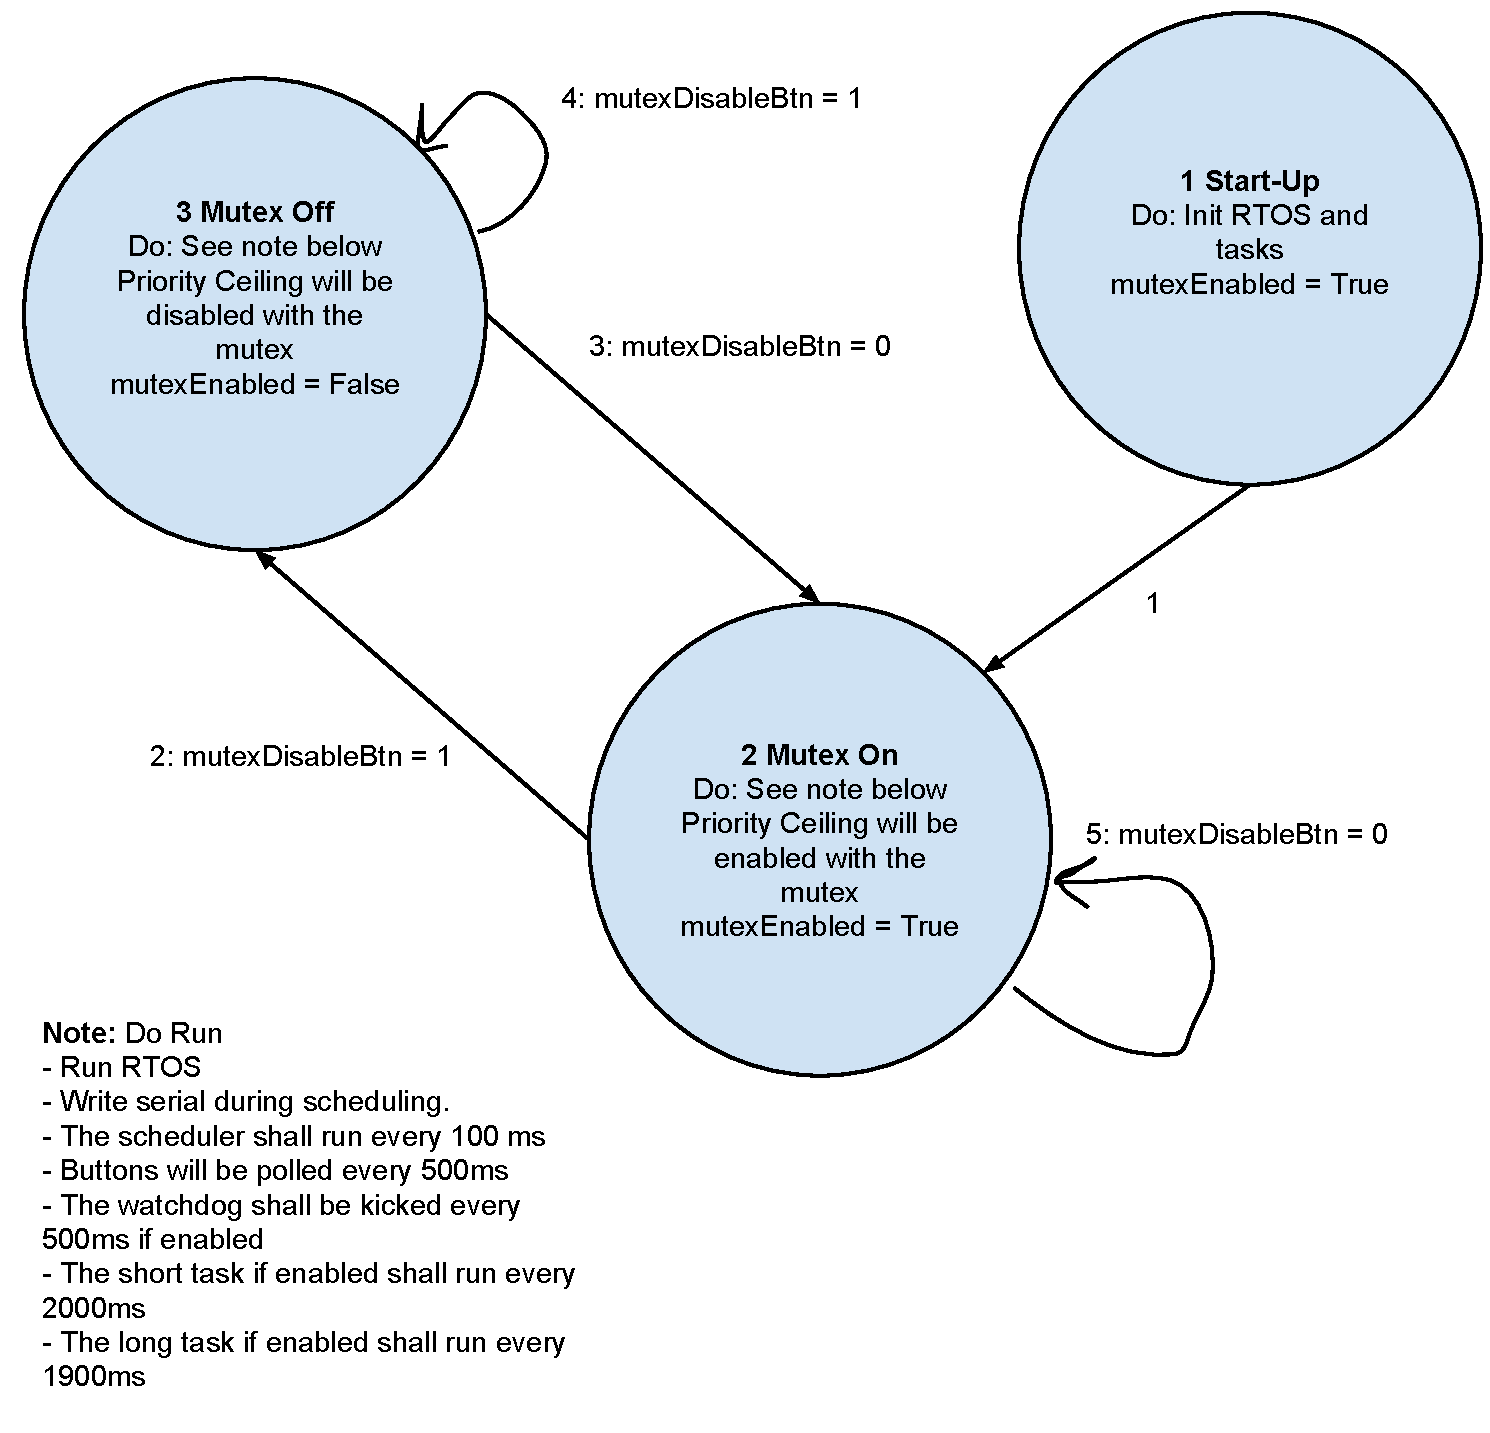
\includegraphics[scale=.5]{RTOS_State_Chart.pdf}
\end{center}

\newpage

\sectPart{Requirements/State-Chart Traceability Table}

NOTE: Because we are implementing an RTOS that majority of our requirements relate to RTOS timing and behavior. RTOS state is not easily encapsulated in a state diagram as its state is based on task timing. The state transition diagram relates to the demonstration and peripherals which function as a result of correct RTOS behavior but do not define the RTOS behavior itself.

\vspace*{1em}

\begin{center}
    \begin{tabular}{| c | c | c | c | c | c | c | c | c |}
        \hline
    Req. & State 1 & State 2 & State 3 & Trans 1 & Trans 2 & Trans 3 & Trans 4 & Trans 5 \\ \hline
    a & - & X & X & - & X & X & X & X \\ \hline
    b & - & X & X & - & - & - & - & - \\ \hline
    c & - & X & X & - & - & - & - & - \\ \hline
    d & - & X & X & - & - & - & - & - \\ \hline
    e & - & X & X & - & - & - & - & - \\ \hline
    f & - & X & X & - & - & - & - & - \\ \hline
    g & - & X & X & - & - & - & - & - \\ \hline
    h & - & X & X & - & - & - & - & - \\ \hline
    i & - & X & - & - & - & - & - & - \\ \hline
    j & X & - & - & X & - & - & - & - \\ \hline
    \end{tabular}
\end{center}

%-----------------------------------------

\sectPart{Scheduling}

The RTOS shall implement and preemptive multitasking with priority ceiling and use this to schedule tasks. It shall use the following priorities and periods:

\vspace{1em}

\begin{center}
    \begin{tabular}{|l|l|l|p{10em}|p{10em}|}
        \hline
        \textbf{Priority} & \textbf{Task} & \textbf{Period (ms)} & \textbf{Description} & \textbf{Timing Rationale} \\ \hline
        N/A & \texttt{scheduler} & 100 & Schedules other tasks. & N/A \\ \hline
        0 & \texttt{kickWatchdog} & 500 & Kicks COP. & Should run with highest priority to avoid tripping COP. \\ \hline
        1 & \texttt{pollSwitches} & 500 & Polls module \texttt{SW3} to determine which other tasks to enable. & Should run with higher priority than most tasks it enables/disables. \\ \hline
        2 & \texttt{shortBlockTask} & 2000 & Grabs the same mutex that \texttt{longBlockTask} wants. & Should run infrequently with long duration so that it is visually observable. \\ \hline
        3 & \texttt{longBlockTask} & 1900 & Grabs the same mutex that \texttt{shortBlockTask} wants. & Should run infrequently with long duration so that it is visually observable. \\ \hline
    \end{tabular}
\end{center}

%-----------------------------------------

\newpage

\sectPart{Watchdog/COP}

When the \texttt{kickWatchdog} task is enabled, it shall kick the watchdog whenever it is run. We shall set COPCTL\_CR = 0x7, so that the watchdog timer will trip if it is not kicked every 1.048576 seconds (assuming an 8 MHz bus clock). \\
Therefore, the watchdog timer will trip if the \texttt{kickWatchdog} task is not scheduled regularly. This would occur if:
    \begin{itemize}
        \item The \texttt{scheduler} does not run regularly or frequently.
        \item The \texttt{scheduler} fails to respect priorities in such a way that \texttt{kickWatchdog} (priority 0) is not scheduled regularly or frequently.
    \end{itemize}
Therefore, if the watchdog trips, we will know that either \texttt{kickWatchdog} is disabled or the scheduler is functioning incorrectly. \\
If the watchdog trips, the RTOS shall shutdown. Then, the demo shall send a message over serial indicating that the watchdog tripped and restart the RTOS.

%-----------------------------------------

\sectPart{Test Plan}

\subsection*{Part 7.1: White Box Testing}

NOTE: Key used to simplify table: M is \texttt{mutexDisableBtn} = 1 and ~M is \texttt{mutexDisableBtn} = 0

\vspace*{2em}

\begin{center}
    \textbf{Tests}\\
    \vspace{0.5em}
    \begin{tabular}{| c | c | c | c | c | c | c |}
        \hline
        Test & Init State & In1 & In2 & In3 & In4 & In5 \\ \hline
        1 & 1 & Any(2) & ~M(2) & M(3) & M(3) & ~M(2) \\ \hline
    \end{tabular}
\end{center}

\vspace*{2em}

\begin{center}
    \textbf{Traceability} \\
    \vspace{0.5em}
    \begin{tabular}{| c | c | c | c | c | c |}
        \hline
        Test & Trans 1 & Trans 2 & Trans 3 & Trans 4 & Trans 5 \\ \hline
        1 & X & X & X & X & X \\ \hline
    \end{tabular}
\end{center}

\newpage

\subsection*{Part 7.2: Black Box Testing}

\begin{center}
    \textbf{Tests} \\
    \vspace{0.5em}
    \begin{tabular}{| c | p{35em} |}
    \hline
    \textbf{Test} & \textbf{Description} \\ \hline
    1 & Run the RTOS and ensure that serial data is being transmitted to the computer \\ \hline
    2 & Record the serial transmission in a log file for each of the following tests. Ensure that the data is in the specified format. Check that the log records the RTOS initialization message and that mutexs are enabled. \\ \hline
    3 & Ensure all the SW3-x start in the off position. Restart the module and ensure that all tasks are disabled in the serial log. \\ \hline
    4 & Look at the logs to ensure that the Watchdog triggers after about 1 second. \\ \hline
    5 & Look at the logs to ensure that the Watchdog event is followed by a software restart. \\ \hline
    6 & Enable the Watchdog Task and restart the module. Press and hold the \texttt{mutexDisable} for 1 second. Check in the log that while \texttt{mutexDisable} was held the module changed the state from \texttt{State 2} to \texttt{State 3} and changed back after the button was released. \\ \hline
    7 & Enable all tasks and restart the module. Run for 1 minute (use a stopwatch) and record logs. \\ \hline
    8 & Look at the logs and ensure all time periods are met for all tasks. Ensure that the scheduler is also meeting its timing. Double check the timestamps which should end at 1 minute. \\ \hline
    9 & Look at the logs and ensure that \texttt{shortBlockTask} and \texttt{longBlockTask} run for the correct duration. \\ \hline
    10 & Look at the logs and find an instance where \texttt{longBlockTask} changes priority. Ensure that this priority is above the priority of \texttt{shortBlockTask} and that \texttt{shortBlockTask} does not run during the execution of \texttt{longBlockTask}. \\ \hline
    \end{tabular}
\end{center}

\vspace*{2em}

\begin{center}
    \textbf{Traceability} \\
    \vspace{0.5em}
    \begin{tabular}{| c | c | c | c | c | c | c | c | c | c | c |}
    \hline
    Test & Ra & Rb & Rc & Rd & Re & Rf & Rg & Rh & Ri & Rj \\ \hline
    1    & -  & -  & X  & -  & -  & -  & -  & -  & -  & -  \\ \hline
    2    & -  & -  & X  & -  & -  & -  & -  & -  & -  & X  \\ \hline
    3    & -  & X  & X  & -  & -  & -  & -  & -  & -  & -  \\ \hline
    4    & -  & X  & -  & -  & -  & X  & -  & -  & -  & -  \\ \hline
    5    & -  & -  & -  & -  & -  & X  & -  & -  & -  & -  \\ \hline
    6    & X  & -  & -  & X  & X  & -  & X  & X  & X  & -  \\ \hline
    7    & -  & -  & X  & -  & -  & -  & -  & -  & -  & -  \\ \hline
    8    & -  & -  & -  & X  & X  & X  & X  & X  & -  & -  \\ \hline
    9    & -  & -  & -  & -  & -  & -  & X  & X  & -  & -  \\ \hline
    10   & -  & -  & -  & -  & -  & -  & -  & -  & X  & -  \\ \hline
    \end{tabular}
\end{center}

%-----------------------------------------

\newpage

\sectPart{Hardware}

Our project shall use the following hardware:
\begin{itemize}
    \item MC9S12C128 microcontroller module (including on-module switches and LEDs)
    \item USB cable (for serial communication)
    \item desktop computer
\end{itemize}
This hardware shall be connected as shown here:\\

\begin{center}
    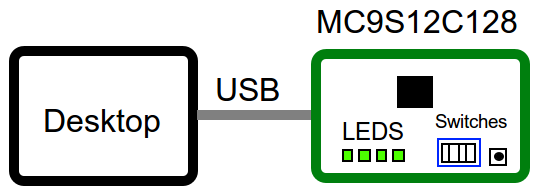
\includegraphics[scale=0.5]{hardware.png}
\end{center}

%-----------------------------------------

\sectPart{Acceptance Test Plan}

The acceptance tests will all involve a Python script which interprets packets with the RTOS sends over serial whenever its scheduler runs. The script will create logs as it runs, which can be checked as part of the acceptance tests. The script's GUI will point out events relevant to the acceptance tests, which will also show up in the logs.
\begin{enumerate}
    \bitem{Test Normal Operation} Run the script for approximately 10 seconds. It will create a log file. In this log file (or by monitering the script's GUI), check that the scheduler lists each task as ``scheduled" at least during each of its periods. Also, check that the message ``WATCHDOG TRIPPED" is not present in the log.
    \bitem{Test Watchdog} Flip SW3-0 to disable the task \texttt{kickWatchdog}. Allow the RTOS to run for at least one second afterward. Observe the script's log file and confirm that ``WATCHDOG TRIPPED" is present at least once.
    \bitem{Test Mutexes (Enabled)} Run the script for approximately 10 seconds. In the log, check for a packet that meets the following criteria:
        \begin{itemize}
            \item Both tasks 2 and 3 (\texttt{shortBlockingTask} and \texttt{longBlockingTask}, respectively) are listed as ``Ready To Run".
            \item Only task 3 is listed as ``Scheduled to Run".
        \end{itemize}
    In this case, the log should also show that task 3 has a higher priority than task 2. This means that task 3 was raised to the mutex's priority ceiling and allowed to run instead of task 2 until task 3 left its critical region.
    \bitem{Test Mutexes (Disabled)} Run the script for approximately 10 seconds, holding \texttt{mutexDisableBtn} the whole time. Check that there is no packet that meets the criteria described in the previous test. This is because task 3 shall never preempt task 2 if priority ceiling is not in place.
\end{enumerate}




%-----------------------------------------

\newpage

\section*{Appendix}

    \subsection*{RTOS API}
        
        Users may start and stop the RTOS using:
        \begin{itemize}
            \bitem{\texttt{void rtosStart(void)}}
            \bitem{\texttt{void rtosShutdown(void)}}
        \end{itemize}

        The RTOS will internally represent tasks using the type \texttt{task\_t}. Users may configure the RTOS's task scheduler using:
        \begin{itemize}
            \bitem{\texttt{void rtosSetSchedulerPeriod(uint16\_t period)}}
            \bitem{\texttt{void rtosSetTaskArray(task\_t[] tasks, uint8\_t numTasks)}}
            \bitem{\texttt{void void rtosAddTask(uint8\_t priority, uint16\_t period, void (*task) (void))}}
        \end{itemize}
        These configuration functions should be called before calling \texttt{rtosStart()}. \\


        Additionally, the RTOS will provide a mutex implementation. Mutexs will have type \texttt{mutex\_t}. The RTOS will support the following functions for mutexes:
        \begin{itemize}
            \bitem{\texttt{rtosAddMutex(uint8\_t priority, mutex\_t *mutex)}}
            \bitem{\texttt{rtosAcquireMutex(mutex\_t *mutex)}}
            \bitem{\texttt{rtosReleaseMutex(mutex\_t *mutex)}}
        \end{itemize}

        Finally, the user may enable and disable various features and tasks while the RTOS is running using the following methods:
        \begin{itemize}
            \bitem{\texttt{void rtosEnableDebug(bool\_t enable)}}
            \bitem{\texttt{void rtosEnableMutexes(bool\_t enable)}}
            \bitem{\texttt{void rtosEnableTask(bool\_t enable)}}
        \end{itemize}
        
%=======================================================

\end{document}
